\documentclass[]{article}
\usepackage{graphicx}
\usepackage{amsmath}

%opening

\begin{document}

\section{Overview of NLP content}
\subsection{Finite State Automata and Regular Expressions}
\begin{itemize}
	\item A finite state automaton (FSA) is a directed graph with a finite number of nodes.

	\item A FSA is described by a 5 tuple: (states, alphabet, initial state, final state, transition)
	
	\begin{figure}[h!]
		\begin{center}
			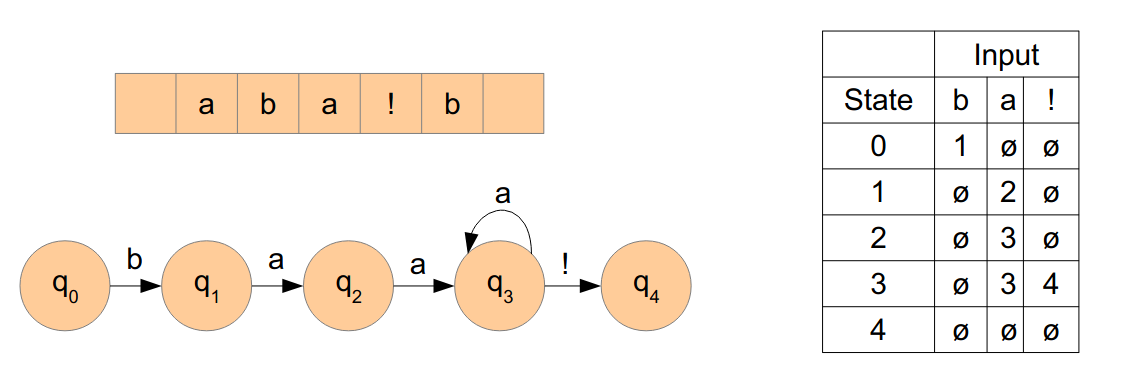
\includegraphics[width=\linewidth]{./images/fsa1.png}
			\label{fig:fsa1}
			\end{center}
	\end{figure}
	
	\begin{center}
	Figure \ref{fig:fsa1}: Example FSA representation
	\end{center}
	

	\item A deterministic FSA is one whose behaviour is fully determined by the state it is in and the input
	

	\item a non-deterministic FSA has an element of stochasticity; perhaps two paths for the same input, or a $\epsilon$ (i.e. spontaneous) transition 
	
	\item NDFSA's present challenges when determinig whether a string should be accepted (by the language) as 'the wrong path' may be taken. A solution to this is to use a backtrack algorithm.
	
	\item Any NDFSA can be converted to a DFSA (See: parallel algorithm)
	
	

\end{itemize}
Regular expressions are a powerful tool for pattern matching. 
They are one way to define an FSA, and also to define a formal (specifically regular) language. Any regular expression can be defined as an NDFSA and hence a DFSA


A formal language is a set of strings that are composed entirely from a finite symbol set $\Sigma$

\subsection{Finite State Transducers}

a FST is a more general function than an FSA. It 'reads' one string and generates another



%\begin{figure}[h!]
%	\begin{center}
%		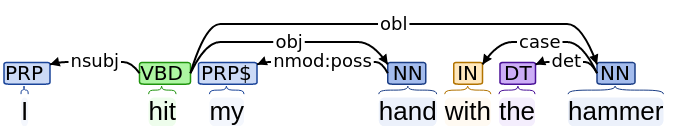
\includegraphics[width=0.6\linewidth]{./images/dependency.png}
%		\label{fig:dep1}
%		\end{center}
%\end{figure}

%\begin{center}
%Figure \ref{fig:dep1}: A typical dependency parse in (CoreNLP parse)
%\end{center}



\end{document}
